\section{Examples}\label{SecExamples}
In this section we illustrate the functioning of the \NAME
library and their interfaces through specific examples, including
discussion of relevant code snippets.
Specifically, we show how the quantum impurity solver in \NAME can be used
to address problems of different nature within the framework of DMFT. 


\subsection{Bethe lattice DMFT (Fortran API)}
The description of the Mott or metal to insulator transition (MIT)
within the Bethe lattice, i.e. Cayley tree with connection
$z\to\infty$ is conventionally considered the test bed of any DMFT
application. Here  we discuss a guided implementation based on the
Fortran API of \NAME of the DMFT solution of the Bethe lattice at
$T=0$. 
We consider a Fermi-Hubbard model:
$$
H = -t \sum_{\langle ij\rangle\s}c^+_{i\s}c_{j\s} + U \sum_i n_{i\up}n_{i\dw}
$$
defined on a Bethe lattice with density of states
$\rho(x)=\frac{1}{2D}\sqrt{D^2-x^2}$, where $D=2t$ is the
half-bandwidth~\cite{Georges1996}.
In DMFT this model is mapped
onto a quantum impurity problem with an effective electronic bath
which needs to be determined self-consistently.
\begin{lstlisting}[style=fstyle,numbers=none,basicstyle={\scriptsize\ttfamily}]
program ed_hm_bethe
   USE EDIPACK2
   USE SCIFOR
   implicit none
   !> Number of discretization points for the Bethe DOS
   integer,parameter                           :: Le=5000
   !> Bethe half-bandwidth = energy unit
   real(8),parameter                           :: D=1d0
   !>Bath:
   real(8),allocatable                         :: Bath(:)
   !> local dynamical functions, rank-5 [Nspin,Nspin,Norb,Norb,L]
   complex(8),allocatable,dimension(:,:,:,:,:) :: Weiss,Smats,Sreal,Gmats,Greal,Weiss_
   ... (omissis)
   !> READ THE input using EDIpack procedure:
   call ed_read_input(trim(finput))
   !
   !> Setup the Bethe DOS $\rho$ (linear dispersion)
   Ene = linspace(-D,D,Le,mesh=de)
   DOS = dens_bethe(Ene,D)
\end{lstlisting}

The bath is described
by the (unknown) function $\GG^{-1}_0$, i.e. the Weiss field. Within \NAME
exact diagonalization approach, where the bath is approximated with a
finite number of levels, the function $\GG^{-1}_0$ is used to
determine bath parameters $\vec{x}=\{V,h\}$ using the optimization method discussed in
\secu{sSecFit}.
The starting point of any calculation is determined by a suitable
guess of the Weiss field, or equivalently of the bath parameters.
In \NAME this operations is accomplished by the function {\tt
  ed\_init\_solver}.

\begin{lstlisting}[style=fstyle,numbers=none,basicstyle={\scriptsize\ttfamily}]
Nb=ed_get_bath_dimension()
allocate(bath(Nb))
call ed_init_solver(bath)
\end{lstlisting}








The iterative algorithm proceeds as follows:
\begin{enumerate}
\item Call the exact diagonalization {\bf impurity solver} {\tt
    ed\_solve} whose only input is the set of parameters $\vec{x}$. All other
  options are controlled by input file specifications ({\tt
    ed\_read\_input}).
\item Retrieve at least the self-energy functions $\Sigma_{\a\b\s\s'}(i\omega)$ on the
  Matsubara axis using {\tt ed\_get\_sigma}.
\item Evaluate the local interacting Green's function
  $G_{loc}(i\omega) = \int_{-D}^D \frac{\rho(\e)}{\zeta -\e}d\e$ with
  $\zeta=i\omega+\mu-h^0-\Sigma(i\omega)$.
  \item Update the Weiss field through the {\bf self-consistency}
    relation: $\GG^{-1}_0(i\omega) = G_{loc}(i\omega) + \Sigma(i\omega)$. 
  \item Optimize the bath parameters $\vec{x}$ against the updated
    Weiss field using, for instance, {\tt ed\_chi2\_fitgf}. Restart at 1.
\end{enumerate}
In agreement with Reverse Communication Strategy setup, the step 3-4
are left to the user. In addition step 5 is kept separated to
guarantee enough freedom in the bath optimization, though we remark
this is a crucial step which can potentially compromise the whole
calculation.
An example of implementation is given in the following listings.

\begin{lstlisting}[style=fstyle,numbers=none,basicstyle={\scriptsize\ttfamily}]
iloop=0;converged=.false.
   do while(.not.converged.AND.iloop<nloop)
     iloop=iloop+1     
     !> Solve the effective impurity problem
     call ed_solve(bath)     
     !> Retrieve impurity Self-energy on Matsubara axis
     call ed_get_sigma(Smats,'m')
     !
     !> Build a local Green's function:
     wfreq = pi/beta*(2*arange(1,Lmats)-1)   !automatic Fortran allocation
     do i=1,Lmats ! One can do better than this of course 
        zeta= xi*wfreq(i)+xmu - Smats(1,1,1,1,i)
        Gmats(1,1,1,1,i) = sum(DOS(:)/( zeta-Ene(:) ))*de  
     enddo
     !> Update Weiss field: Self-consistency
     Weiss(1,1,1,1,:) = one/(one/Gmats(1,1,1,1,:) + Smats(1,1,1,1,:))
     !> Close the self-consistency fitting the new bath:
     call ed_chi2_fitgf(Weiss,bath,ispin=1)     
     !>Check convergence
     converged =( sum(abs(Weiss(1,1,1,1,:)-Weiss_(1,1,1,1,:)))/sum(abs(Weiss(1,1,1,1,:))) )<dmft_error
     Weiss_=Weiss     
   enddo
\end{lstlisting}


\subsubsection{Results}
In the following we present some results obtained by executing this
simple program varying the interaction strenght :f:var:`uloc`.
Differently from the previous case of a quantum impurity embedded in a
given bath describing the progressive formation of a
strongly renormalized Fermi liquid state, here the DMFT
self-consistency allows to describe the transition from a correlated
metal to a Mott insulating state.


To illustrate this point, in panel **A** we report the evolution of
the spectral function $-{\rm Im}G(\omega)/\pi$ as a function of
$U$. Despite the *spiky* nature of the spectrum, due to the
finite size (i.e. number of poles) of the discretized effective bath,
one can clearly distinguish the renormalization of the central
quasi-particle peak at low-energy and the concomitant formation of
rather incoherent  high-energy features which will develop into
Hubbard bands for $U>U_c$, with $U_c\simeq 2.8D$. 


\begin{figure}[t!]
  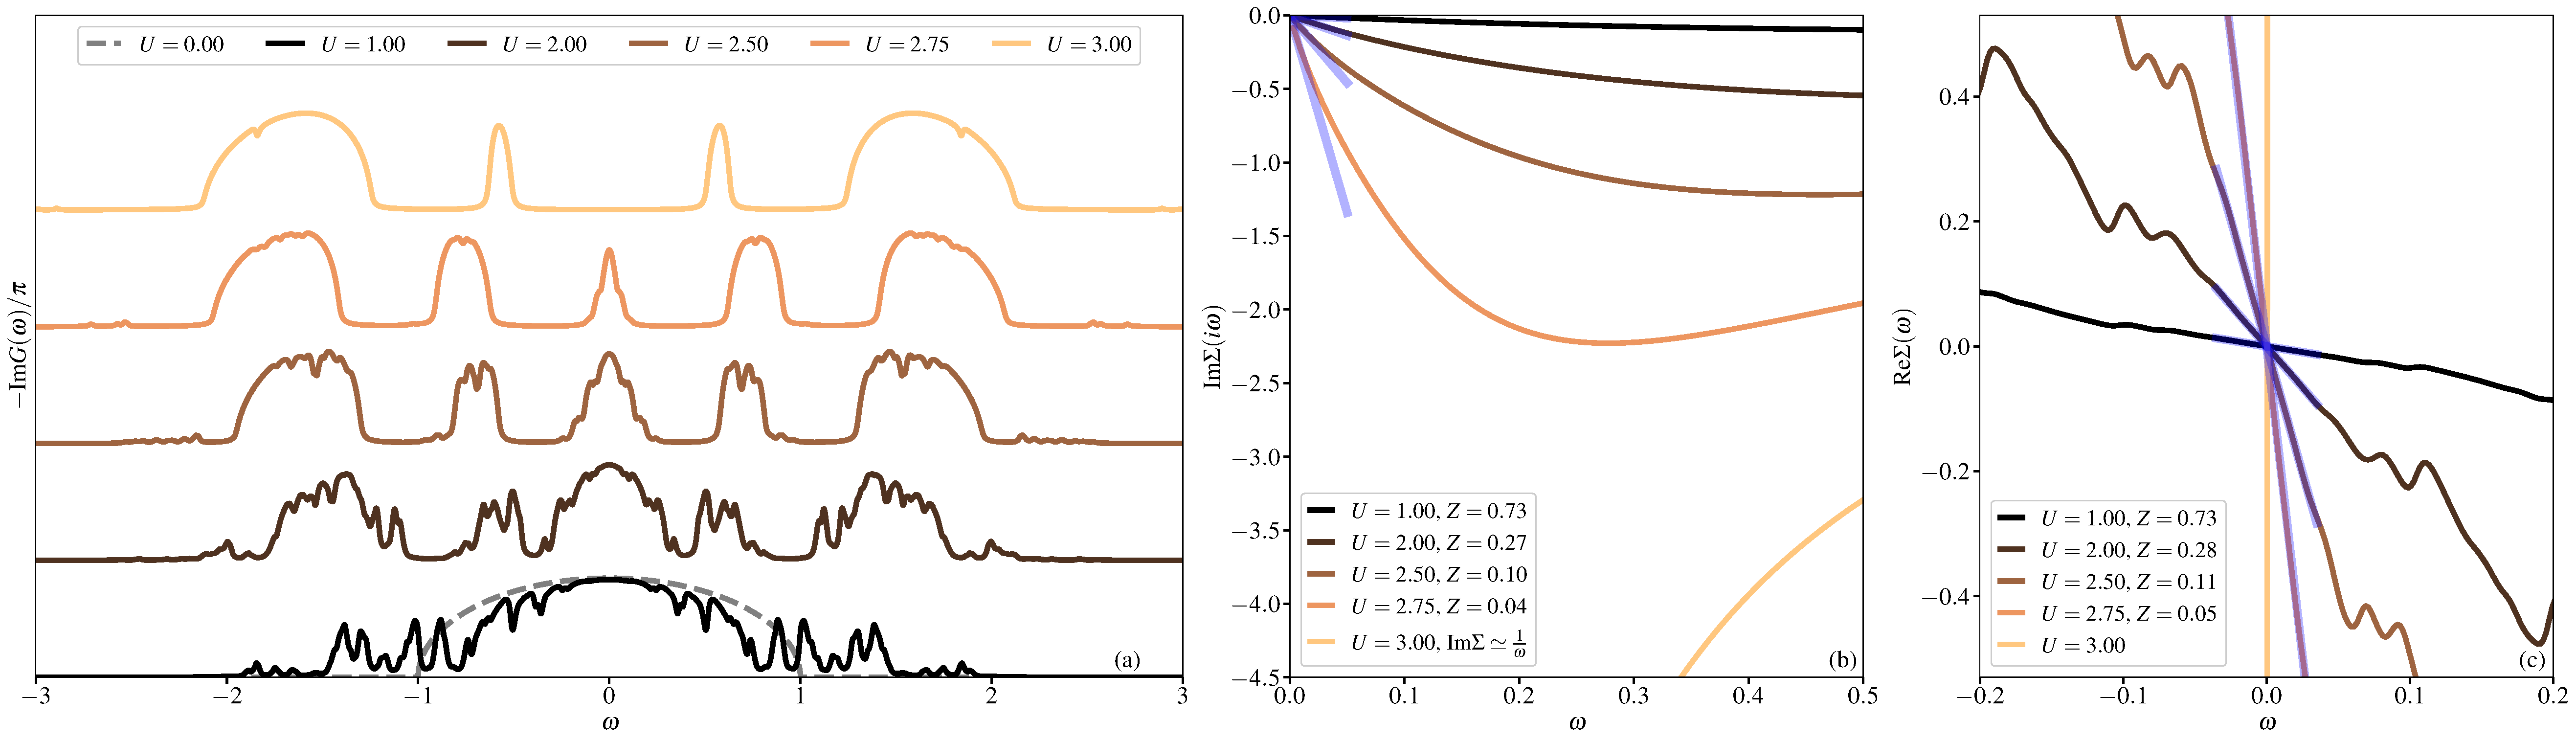
\includegraphics[width=\linewidth]{figures/figBethe.pdf}
    \caption{\label{fig1}%
        \textbf{The Mott transition.}
        }
\end{figure}



In the panels (B) and (C) we further discuss the metal-insulator
transition by showing the evolution of the self-energy functions.
In panel (B) we report the self-energy ${\rm Im}\Sigma(i\omega)$
on the Matsubara axis in the low energy regime. Increasing $U$
we observe the progressive growth of this function until it takes a
diverging behavior crossing the critical interaction strenght. We
recall that this behavior can be observed on the Matsubara axis
because of the particle-hole symmetry of the problem.

Using the relation:

$$
   \frac{\Im\Sigma(i\omega_n)}{\omega_n}_{|_{\omega_n\rightarrow 0}}=
   \frac{1}{\pi}\int_{\mathbb R}d\epsilon \frac{\Re\Sigma(\epsilon)}{\epsilon^2}=
   \frac{\partial\Re\Sigma}{\partial\omega}_{|_{\omega\rightarrow 0}}.
$$
we can extract the quasi-particle renormalization constant :math:`Z`
from the linear behavior of ${\rm Im}\Sigma(i\omega)$ near
$\omega=0$ in the metallic regime. The results are highlighted
in the figure and the values of $Z$ are reported in the legend.

Using the right hand side of the previous relation, we show in
panel (C) the behavior of  ${\rm Re}\Sigma(\omega)$
on the real axis around the Fermi level. Again, increasing $U$
we observe the slope of the linear behavior to increase until the
critical point is crossed and an insulating state is reached. On the
real-axis this is signaled by the divergence of the imaginary part of
the self-energy   ${\rm Im}\Sigma(\omega) \rightarrow -\infty$
near the chemical potential, which here is set to zero by
particle-hole symmetry. The corresponding real part shows a
discontinuity visibile in the panel (C). 


\subsection{Attractive Hubbard model (Python API)}
The second application has the twofold aim to demonstrate the
superconductivity support of the \NAME library as well as to
illustrate the Python API through a working example.



\subsection{Multi-orbital Hubbard (Triqs)}

\subsection{Some model (W2Dynamics)}

\subsection{Interacting Bernevig-Hughes-Zhang (Fortran)}

